%%%%%%%%%%%%%%%%%%%%%%%%%%%%%%%%%%%%%%%%%%%%%%%%%%%%%%%%%%%%%%%%%%%%%
%%                                                                 							%%
%%		Trabajo Fin de GRADO		                       				%%
%%		TITULO 																			%%
%%		AUTOR												%%
%%                                                                 							%%
%%%%%%%%%%%%%%%%%%%%%%%%%%%%%%%%%%%%%%%%%%%%%%%%%%%%%%%%%%%%%%%%%%%%%

%%  Include con la definicion de estilos por el usuario
%%%%%%%%%%%%%%%%%%%%%%%%%%%%%%%%%%%%%%%%%%%%%%%%%%%%%%%%%%%%%%%%%%%%%

\input definl

%%  Paqueteria necesaria de fabrica
%%%%%%%%%%%%%%%%%%%%%%%%%%%%%%%%%%%%%%%%%%%%%%%%%%%%%%%%%%%%%%%%%%%%%
\usepackage{hyperref}
\usepackage{palatino}
\usepackage[dvips]{graphicx} 	  % para importar combinados latex
\usepackage{color}          		      % para importar dibujos coloreados
\usepackage{rotating}        		  % para usar \begin{sideways} que rota tabla 90 grados 
\usepackage{epsfig}          		  % para rotar figuras de Xfig  poniendo % \begin{sideways} 
\usepackage{amsmath}         	  % para usar matrix y pmatrix environment
\usepackage{stmaryrd}        		  % para usar la \bigsqcap
\usepackage{verbatim}        		  % para poner salidas de pantallas
\usepackage{listings}       	 	  % para imprimir codigo fuente
\usepackage{shortvrb}				  % 
\usepackage{url}						  % 
\usepackage{subfigure}			  % 

  

%%%%%%%%%%%%%%%%%%%%%%%%%%%%%%%%%%%%%%%%%%%%%%%%%%%%%%%%%%%%%%%%%%%%%
%%  Configuracion de paquetes
%%%%%%%%%%%%%%%%%%%%%%%%%%%%%%%%%%%%%%%%%%%%%%%%%%%%%%%%%%%%%%%%%%%%%
\renewcommand\lstlistingname{Listado}                   %  default is Listing
%\renewcommand\lstlistlistingname{\'Indice de listados}  %  default is Listings 
%\renewcommand\thelstlisting{\thechapter .\arabic{lstlisting}} % captionstyle


\lstset{
  language=Java,
  basicstyle=\small,
  keywordstyle=\bfseries,
  showstringspaces=false,
  numbers=left, 
  numberstyle=\tiny, 
  stepnumber=1, 
  numbersep=5pt,
  frame=single}


%%  Configuraciones varias
%%%%%%%%%%%%%%%%%%%%%%%%%%%%%%%%%%%%%%%%%%%%%%%%%%%%%%%%%%%%%%%%%%%%%
\newcommand{\corregir}{\color{blue}}  	 	% pintar en color azul
\setlength{\parskip}{2ex}              			% despues del parrafo, doble linea


% Para que no aparezcan las cabeceras de las páginas que están en blanco
%%%%%%%%%%%%%%%%%%%%%%%%%%%%%%%%%%%%%%%%%%%%%%%%%%%%%%%%%%%%%%%%%%%%%
\makeatletter 
\def\cleardoublepage{\clearpage\if@twoside \ifodd\c@page\else
  \hbox{} 
  \thispagestyle{empty} 
  \newpage
  \if@twocolumn\hbox{}\newpage\fi\fi\fi} 
\makeatother

%%  Cortes de palabras especiales
%%%%%%%%%%%%%%%%%%%%%%%%%%%%%%%%%%%%%%%%%%%%%%%%%%%%%%%%%%%%%%%%%%%%%
\hyphenation{
ejem-plo Algo-ritmo
}


%\includeonly{titulo, prologo,intro,capitulo1}


\begin{document} 

%%  Titulo e Indices
%%%%%%%%%%%%%%%%%%%%%%%%%%%%%%%%%%%%%%%%%%%%%%%%%%%%%%%%%%%%%%%%%%%%%%
\pagenumbering{roman}
\thispagestyle{empty}

{


\thispagestyle{empty}
\begin{center}

\includegraphics[scale=.6]{img/logouhu}
\end{center}

\vspace*{0cm}
\Large 

\begin{center}

{\normalsize \sc Escuelta Técnica Superior de Ingeniería \\ de la Universidad de Huelva}

{\large \bf Grado en Ingeniería Informática}

\vspace*{1cm}

{\sc Trabajo Fin de Grado}


{\LARGE \bf Generación procedimental de mapas 2D. \\ Análisis e investigación del problema. }

\end{center} 




\vfill

\begin{center}
{\normalsize Autor: \\ {\bf Alejandro Seguí Díaz}}
\end{center}

\begin{center}
%{\footnotesize Tutores:}
{\small Tutores: }
\vspace*{0.2cm}
{\small \\  Gonzalo A. Aranda Corral \\ Daniel Márquez Quintanilla}
\end{center}
\begin{center}
{\footnotesize Huelva, 30 de junio de 2015.\\Curso académico 2014/15.}
\end{center}

\newpage
\thispagestyle{empty}
\vspace*{3.5cm}
\begin{center}
\small Puede encontrar una copia actualizada de este documento en \\
\small http://alesegdia.github.io/dungen-docs/latex/src/tfg\_dungen.pdf
\end{center}
\vfill


\newpage
\thispagestyle{empty}
\vfill



}


\clearpage
\pagestyle{plain}
\tableofcontents
\clearpage
\listoffigures

%%  Contenido del trabajo
%%%%%%%%%%%%%%%%%%%%%%%%%%%%%%%%%%%%%%%%%%%%%%%%%%%%%%%%%%%%%%%%%%%%%%
\pagenumbering{arabic}
\pagestyle{fancy}

%\chapter*{Prólogo}
\label{intro:prologo}
\addcontentsline{toc}{chapter}{Prólogo}


\chapter*{Introducción}
\label{intro:intro}
\addcontentsline{toc}{chapter}{Introducción.}

En la actualidad, los videojuegos han conseguido posicionarse en un mercado líder indiscutible a nivel internacional. En el ámbito del entretenimiento, la industria cinematográfica está dando paso a los videojuegos, que avanzan a pasos de gigante. Muchas grandes personalidades del cine se dirigen a los creadores de videojuegos para continuar su carrera. Un ejemplo claro de una persona adelantada para su época en este sentido, es George Lucas (\cite{lucasarts}), autor de la famosa saga Star Wars. George Lucas se introdujo en el mercado de los videojuegos en el 1986 con el título Labyrinth, dando paso posteriormente a otros títulos muy sonados y de culto como Monkey Island o Grimm Fandango.

Un videojuego, al igual que una película, puede contar una historia. Aún así, existen diferentes géneros de videojuegos, que van desde simulación de juegos de mesa, donde evidentemente no existe historia, o está intrínseca en el origen del mismo juego, hasta las denominadas aventuras gráficas, donde el enfoque está en la parte argumental. Es por ello que la industria del cine deja paso a los videojuegos de manera tan rápida.

\section*{Mapas y escenarios.}
\addcontentsline{toc}{section}{Mapas y escenarios}

Muchos géneros de videojuegos plantean su argumento en un escenario donde se da rienda suelta a la capacidad perceptiva del jugador, dando lugar en mayor o menor medida a que complete la historia con su imaginación. En este escenario, el jugador desarrollará las acciones que se le ofrezcan según el tipo de juego. Así, podrá completar la historia, permitiendo además en muchos casos que las acciones influyan en el desarrollo argumental del videojuego. Tipos de juegos que requieren mapas son, por ejemplo, juegos de acción, estrategia o rol entre otros.

El tipo de escenario que podemos encontrarnos en un juego es de lo más variopinto. A la hora de plantear la elaboración de un juego, se tiene en cuenta la elección del tipo de escenario. Muchas cuestiones sobre las que se basan estas elecciones radican sobre la complejidad de optimización del mismo:

\begin{itemize}
	\item Si el escenario es demasiado grande, no nos interesa renderizar el escenario completo, sino solamente la parte visible. Al proceso de optimizar el renderizado del mapa se le llama \emph{culling}\cite{culling}.
	\item Lo mismo pasa con las físicas. No nos interesa comprobar colisiones con elementos que es obvio que no van a colisionar. Ésto también ha de ser tenido en cuenta a la hora de elaborar el sistema de escenarios.
	\item El \emph{nivel de detalle} (Level of detail por el inglés \cite{lod}) es otro aspecto a tener en cuenta. Si una geometría está demasiado lejana del jugador, no necesitamos renderizarla exactamente como es. Este aspecto es relevante a los juegos 3D principalmente.
	\item La división o no del escenario por zonas. Esto puede evitarnos la necesidad de presencia en memoria de un mapa completo, pudiéndolo dividir en partes para ahorrar en el preciado recurso que es la memoria. Es un aspecto a tener en cuenta sobre todo cuando se elaboran juegos para videoconsolas, las cuales suelen contar con una memoria muy limitada.
\end{itemize}

Así, se exponen dos criterios principales como forma de clasificar los tipos de escenario:

\begin{itemize}
	\item Organización del escenario. Este criterio se refiere a la existencia de cortes en el desarrollo del juego para la carga de las distintas partes del mundo en el que se desarrolla el juego. Algunos tipos son:
	\begin{itemize}
		\item Escenarios totalmente continuos continuos representando un mundo totalmente abierto sin cortes. Ejemplos son \emph{GTAV} o \emph{Minecraft}.
		\item Dividido por zonas donde no existen cortes en la misma zona. Un ejemplo es \emph{Borderlands}.
		\item Dividido por zonas donde pueden existir cortes en la misma para interiores. Un ejemplo es \emph{Skyrim}.
	\end{itemize}
	\item Composición del escenario. Nos referimos a si la geometría empleada ayuda de forma implícita al manejo a nivel computacional del escenario. Algunos tipos son:
	\begin{itemize}
			\phantomsection \label{maptiles-r}
		\item Escenarios en 2D discretizados en \emph{tiles}. Básicamente, la geometría está representada por una matriz de dos dimensiones, donde cada casilla de la matriz está relacionada con una textura (o porción de la misma), siendo todas las texturas del mismo tamaño para la misma matriz. A cada casilla, la denominamos \emph{tile}. Este tipo de escenarios son muy fácilmente optimizables. Ejemplos de este tipo es, por ejemplo, \emph{Final Fantasy VI}, así como multitud de juegos de las consolas de 8 y 16 bits como la \emph{NES} o \emph{SNES}.
		\item Una extensión a 3D de los escenarios de tiles son los escenarios compuestos por \emph{voxels} \cite{voxel}. Estos han sido recientemente popularizados por el famoso título \emph{Minecraft}, donde el escenario está gestionado por un \emph{motor de voxels} que ayuda a optimizar tanto con culling como con físicas.
		\item Escenarios con geometría deliberada. Es decir, la geometría (ya sea 2D o 3D), no presenta ninguna propensión a ser optimizada. Este tipo de escenarios, suelen optimizarse con el uso de \emph{quadtrees} \cite{quadtree} (para 2D) u \emph{octrees} \cite{octree} (para 3D)
		\item Escenarios hechos con los denominados \emph{brushes} \cite{brush}. Esta técnica se utiliza para 3D, y consiste en el uso de geometrías convexas para componer un escenario. Ejemplos famosos de este tipo de escenarios es \emph{Quake} \cite{quake}.
	\end{itemize}
\end{itemize}

Una vez expuestos los criterios para clasificar los tipos de mapas, remarcar que hay casos en los que los desarrolladores convienen formas nuevas de organizar el mapa debido a necesidades particulares, por lo que los ejemplos expuestos en cada criterio no completan de ninguna manera las múltiples categorías para cada uno.

Para el desarrollo de este proyecto y atendiendo a las especificaciones presentadas en el capítulo~\ref{cap:capitulo2}, abarcaremos \emph{mapas de tiles} para el género de juego \emph{roguelike} \cite{rlike}. Este género se caracteriza precisamente por mapas generados de forma procedimental. Cada nivel es entendido como una planta, donde el jugador tiene que llegar desde donde aparece hasta un tile considerado como final para poder continuar hasta la siguiente planta. Así, el jugador va avanzando niveles hasta que llega al último y completa el juego al finalizar el mismo.



\section*{Motivación y Objetivos.}
\addcontentsline{toc}{section}{Motivación y Objetivos}

Como se ha mencionado previamente, la industria de los videojuegos avanza a pasos de gigante. Es por ello que las compañías invierten cada vez más en videojuegos, siendo a veces el coste en marketing superior al de desarrollo \cite{costgames}. Existe un amplio espectro de puestos encontrados en este campo \cite{gdroles1} \cite{gdroles2}, entre los cuales existen

\begin{itemize}
	\item \emph{Game programmer}. Personal dedicado a la programación de las mecánicas del juego, eventos y otros relacionados con el propio juego
	\item \emph{Core programmer}. Personal dedicado a la elaboración del motor que será la base sobre la que funcionará el juego. Normalmente se subdivide en subroles como \emph{graphics programmer} o \emph{physics programmer}. En muchos casos, se parte de un motor ya elaborado sobre el que se realizan las modificaciones necesarias para el juego en cuestión.
	\item \emph{Game designer}. Dedicados a la elaboración de las mecánicas del juego, así como el plot del mismo.
	\item \emph{Level designer}. Personal dedicado exclusivamente a la elaboración de escenarios empleando programas externos o el mismo motor que se esté utilizando, si éste posee dichas capacidades.
	\item \emph{AI programmer}. Dedicado a la programación de los distintos sistemas de inteligencia artificial existentes en el juego.
	\item \emph{Muchos más...}
\end{itemize}

En este listado, solo hemos tenido en cuenta algunos de los puestos del aspecto de desarrollo, pero quedaría añadir muchos más como diseñadores gráficos y apartado de marketing.

Destacar que el \emph{level designer}, pese a que no se encarga de la construcción de las herramientas para crear el escenario, debe conocer las bases del tipo de escenario que se empleará en el juego, de forma que adapte sus técnicas de diseño al tipo de escenario y así poder optimizarlos en la medida de lo posible.

Recientemente, y debido a las cada vez más crecientes facilidades para crear un videojuego, han surgido los llamados \emph{equipos indies} \cite{gdindie}, caracterizados principalmente por tener un bajo presupuesto y personal. Normalmente suelen empezar con un presupuesto nulo, pero en algunos casos llegan a triunfar de manera inesperada incluso por los mismos desarrolladores. Ejemplos son \emph{Hotline Miami}, \emph{Minecraft} o \emph{Risk of Rain}.

Los equipos con un presupuesto considerable (coloquialmente denominados AAA), no tienen problemas a la hora de contratar \emph{diseñadores de niveles}, ya que disponen de una gran cantidad de dinero para depositar en los distintos roles necesarios para un juego. Aún así, en combinación con un generador de mapas, un \emph{diseñador de niveles} puede desarrollar ideas que den un resultado muy bueno. Ejemplos de esto son \emph{Diablo} o \emph{Torchlight}, donde los mapas son generados automáticamente partiendo de patrones elaborados a mano por \emph{diseñadores de niveles}.

Así, el la motivación de este proyecto reside en dos ideas principales.

\begin{itemize}
	\item Ahorro de coste y tiempo para equipos indies, que no pueden permitirse el lujo de gastar en personal exclusivo para el diseño de niveles.
	\item Adición de variedad a los escenarios de juegos, permitiendo incluso a un equipo de desarrolladores AAA
\end{itemize}


\section*{Solución Propuesta.}
\addcontentsline{toc}{section}{Solución Propuesta}

La solución que se propone es un sistema capaz de generar escenarios de manera automática con una mínima interacción (o incluso nula si se desea) de los diseñadores. Esto además, conlleva dinamismo en los escenarios que se podrán jugar, de forma que de partida a partida, la distribución del escenario será completamente distinta.

La elaboración de un generador de escenarios, une las competencias de dos roles en el desarrollo de videojuegos:

\begin{itemize}
	\item \emph{Diseñador de niveles.} Se necesitan conocimientos sobre la composición de los escenarios del juego, además de las propiedades concretas en cuanto a los criterios mencionados anteriormente.
	\item \emph{Programador de IA}. La creación del sistema que genere los escenarios es un trabajo que compete a este rol, ya que estamos tratando de resolver un problema donde las posibilidades de resolución son casi infinitas.
\end{itemize}

Finalmente, se elaborará el sistema reduciendo el problema a una búsqueda, donde el \emph{espacio de estados} son todas las posibles combinaciones de habitaciones conectadas.

\section*{Estructura de la memoria.}
\addcontentsline{toc}{section}{Estructura de la memoria}

Esta memoria se estructura en varios capítulos, con la siguiente distribución de los temas trabajados:

\begin{itemize}
	\item Capítulo~\ref{cap:capitulo1}. Mostraremos el origen y estado actual del campo de generación procedimental de contenido.
	\item Capítulo~\ref{cap:capitulo2}. Definiremos el problema junto con sus especificaciones y requisitos. Se comentará el tipo de juego al que se ha enfocado y el tipo de mapa utilizado.
	\item Capítulo~\ref{cap:capitulo3}. Analizaremos en profundidad la representación del modelo de datos elegida para el desarrollo del generador propuesto.
	\item Capítulo~\ref{cap:capitulo4}. Desarrollo de la estrategia empleada para el generador. Como se podrá comprobar, se ha utilizado una estrategia flexible sobre la que posteriormente, construiremos el método de búsqueda.
	\item Capítulo~\ref{cap:capitulo5}. Detalle de la implementación basada en búsqueda. Analizaremos cada uno de los elementos empleados tanto para la generación del mapa, como para la adición de diversidad.
	\item Capítulo~\ref{cap:capitulo6}. Una vez explicada la estrategia, en este capítulo se desarrollará una correspondencia entre el método de búsqueda y la estrategia implementada basada en el mismo.
	\item Capítulo~\ref{cap:capitulo7}. Comparación y análisis del impacto de diversos componentes que se han empleado para promover tanto la diversidad como la eficiencia.
	\item Capítulo~\ref{cap:capitulo8}. Posible trabajo futuro pertinente a la elaboración de una aplicación comercial con el método expuesto en este proyecto
	\item Bibliografía.
\end{itemize}

\chapter{Estado del arte.}\label{cap:capitulo1}

En este capítulo, analizaremos el ámbito de la generación procedimental de contenido para videojuegos. Veremos las distintas subdisciplinas presentes, así como los problemas que resuelven. Se hará hincapié en la generación de escenarios, ya que es el campo que compete al proyecto.

\section{Generación de contenido procedimental.}

Más conocida por su nombre en inglés (Procedural Content Generation), se refiere a la disciplina de generar contenido partiendo de algoritmos, en lugar de hacerlo manualmente.

Tuvo sus inicios en la subcultura informática llamada \emph{Demoscene} \cite{dmscn}. Este movimiento tuvo sus inicios a finales de los años 70 y principios de los 80, y continúa a día de hoy. Consiste en crear contenido visual y sonoro de forma programada, ya sea en parte o en su totalidad, y tenía como uno de sus objetivos escudriñar al máximo las limitadas capacidades de los ordenadores de la época.

Los \emph{sceners} de este campo, conseguían generar contenidos que eran impensables para la época, como por ejemplo escenas en 3D cuando a OpenGL aún le quedaban un par de décadas para aparecer. Por su habilidad, la mayoria de los demosceners terminaban trabajando para empresas de videojuegos de la época, cuando aún no había tantas facilidades a la hora de crearlos.

Existen diversas subdisciplinas en las que se aplica el concepto de generación procedimental de contenido:

\begin{itemize}
	\item \emph{Escenarios}.
	\item Texturas \cite{texmodproc}. Un ejemplo de ello es la generación de texturas que imitan el mármol o la madera. En algunos casos se emplean autómatas celulares.
	\item Geometría. Generación de follaje, o árboles empleando L-Systems. \cite{texmodproc}
	\item Mecánicas. El juego Left4Dead y su secuela, emplean un sistema procedimental para gestionar los momentos de tensión y la dificultad de las situaciones según las acciones que han ido tomando los jugadores.
\end{itemize}

Otra clasificación de los métodos procedimentales es según el momento de ejecución del procedimiento. Si el procedimiento es ejecutado antes del lanzamiento del juego, o después con la particularidad de que se realiza en servidores ajenos al jugador, lo denominaremos \emph{offline}. Sin embargo, si el procesamiento se realiza en el sistema en que se está ejecutando el juego, lo llamaremos \emph{online}.

\section{Generación de mapas.}

La generación de escenarios se considera un concepto muy amplio, ya que según el contexto del juego, puede variar bastante. Por ejemplo, en un juego ambientado en el espacio exterior, el escenario puede entenderse como una galaxia completa, como es el caso de \emph{Elite: Dangerous}.

Otro tipo de modelo a usar en la generación de escenarios es el ruido Perlin. Éste puede ser muy útil en conjunto con el concepto de mapas de alturas para generar terrenos al aire libre montañosos \cite{libnoise}. También se ha empleado el \emph{algoritmo de Voronoi} para la generación de terrenos \cite{amitvoronoi}.

Algún ejemplo más histórico de generación de escenarios pueden ser los múltiples algoritmos de generación de laberintos que se conocen \cite{labygen}.

Debido a que los métodos anteriores son demasiado genéricos, una opción muy popular es idear y construir un generador específico para el juego en cuestión que se esté desarrollando. Un ejemplo de ello es \emph{TinyKeep}, cuyo autor describe a grandes rasgos en \cite{tinykeep} las fases y el desarrollo del algoritmo que ha creado. Esta opción es la que se desarrollará en este proyecto, procurando mantener un nivel de genericidad y capacidad de personalización del sistema.



   % 
\chapter{Especificaciones.}\label{cap:capitulo2}

Definiremos las especificaciones y directrices tanto del tipo de juego como del sistema de generación. Dichas directrices que delimitarán el sistema a crear, han sido establecidas por la empresa indie de videojuegos \emph{TheGameKitchen}, y el sistema será empleado en un futuro título de la misma.

\section{Género de juego.}

En esta sección abarcaremos el tipo de juego y las directrices establecidas en cuanto al género de juego y otras especificaciones relacionadas con el mundo en el que se desarrollará el mismo.

\subsection{Roguelike}

El género de juego en el que nos basaremos será \emph{roguelike} \cite{rlike}, cuyas características principales son:

\begin{itemize}
	\item \emph{Generación de mazmorras}. Cada vez que el jugador inicia una partida, la experiencia será ligeramente distinta.
	\item \emph{Importancia considerable a la exploración}. El hecho de que las mazmorras no sean siempre iguales, incita al jugador a tener que invertir tiempo en explorar para poder encontrar la salida.
	\item \emph{Desarrollo del juego por plantas}. El objetivo del jugador suele ser llegar a una habitación considerada como final, donde puede elegir entre tomar las escaleras para pasar a una siguiente planta, o investigar un poco más en la presente.
	\item \emph{Dificultad progresiva}. Cada planta, tendrá una dificultad ligeramente mayor a la de la anterior hasta llegar a la última.
	\item \emph{Muerte permanente}. Una vez que el jugador muere, no hay manera de cargar la partida. La unica opción es comenzar de nuevo.
\end{itemize}

Históricamente, el género \emph{roguelike} se identificaba además por otro tipo de características, como la mecánica por turnos o el énfasis en jugabilidad y desinterés en los gráficos, pero con el tiempo, el género se ha ido abriendo paso a una definición más genérica. Debido a ésto, hoy en día existen desde \emph{shooters} considerados \emph{roguelike}, como por ejemplo \emph{Tower of Guns} o \emph{Paranautical Activity}, hasta \emph{plataformas}, como \emph{Risk of Rain} o \emph{Spelunky}.

\subsection{Especificaciones del mundo}

Así, las únicas especificaciones que se han dado en cuanto a las reglas de juego son las siguientes:

\begin{itemize}
	\item Entorno en dos dimensiones
	\item El jugador comenzará en una habitación y tendrá como objetivo llegar a una habitación final
	\item Se empleará una vista cenital (figura~\ref{fig:tileclip}).
\end{itemize}

\begin{figure}[t]
\centering
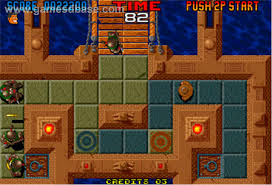
\includegraphics[scale=1]{img/cenital}
\caption{Vista cenital en el juego Action Hollywood por TCH, 1995
\label{fig:cenital}}
\end{figure}

Estas especificaciones son bastante genéricas, por lo que el sistema elaborado podrá servirnos para otro tipo de juegos. Más adelante veremos que se ha procurado dar un enfoque de alta flexibilidad en este aspecto al sistema.

\section{Requisitos del escenario.}

La representación de los escenarios elegida será un mapa de tiles. Como se comentó anteriormente, los mapas de tiles están representados por una matriz, donde cada casilla corresponde a un gráfico de un tamaño normalizado para todos los tiles (un gráfico para las paredes, otro para el suelo, etc). Suelen componerse por capas para añadir decorado, pero para nuestra finalidad, hemos obviado esta característica, ya que se hará hincapié principalmente en la distribución de las habitaciones. No obstante, sería muy sencillo añadir capas como mejora futura.

La optimización en cuanto a clipping (evitar renderizar zonas no visibles) en un mapa de tiles está muy investigada. Debido a que el propio mapa es una rejilla, se puede recorrer y renderizar exclusivamente la zona que va a verse. En la figura~\ref{fig:tileclip} se representa en rojo el viewport del jugador. Los tiles amarillos están en el borde del viewport, y los verdes están completamente dentro. Así, solo hace falta recorrer y dibujar los tiles verdes y amarillos, ahorrándonos el dibujado de los azules.

\begin{figure}[t]
\centering
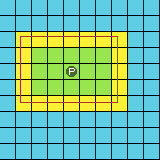
\includegraphics[scale=1]{img/tileclip}
\caption{Clipping en un mapa de tiles
\label{fig:tileclip}}
\end{figure}

Otra característica importante de los mapas de tiles es la sencillez y flexibilidad que da a la hora de componer escenarios; podemos reutilizar tiles y añadir variaciones de los mismos para, en el mapa final, dar sensación de variedad sin tener que elaborar muchos gráficos.

Por todo ello, es un tipo de escenario muy popular desde las antiguas consolas como \emph{NES} o \emph{SNES} hasta hoy.

El escenario estará compuesto por habitaciones, cada una representada como una matriz. Será nuestra tarea plantear un sistema que elabore distribuciones de las habitaciones según los requisitos que se expondrán a continuación.

\section{Directrices para la generación.}

En esta sección explicaremos las directrices impuestas para la generación de los escenarios.


\subsection{Lista inicial de habitaciones}

El sistema que construiremos deberá cumplir una serie de características que analizaremos en detalle en esta sección. Como se ha mencionado previamente, se ha tomado la libertad de añadir características que no estaban en los requisitos previos de \emph{TheGameKitchen}.

El sistema debe generar un mapa de tiles partiendo de una \emph{lista inicial de habitaciones} previamente construida. Para construir las habitaciones, se ha elaborado un editor via web usando el canvas que proporciona HTML y JavaScript (se puede ver en la figura~\ref{fig:roomed}). Así, el objetivo será colocar las habitaciones presentes en esta lista inicial.

\begin{figure}[t]
\centering
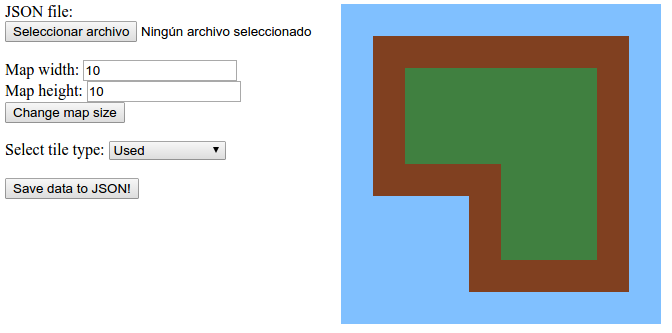
\includegraphics[scale=0.5]{img/roomed}
\caption{Editor de habitaciones
\label{fig:roomed}}
\end{figure}

Las habitaciones \emph{pueden repetirse}, es decir, si hemos creado dos modelos de habitación \emph{A} y \emph{B}, podemos tener 3 instancias del modelo \emph{A} y 2 instancias del modelo \emph{B} en la lista inicial. Hablaremos de este detalle en el próximo capítulo, que nos servirá para conseguir una mejora de optimización tanto de memoria como en procesamiento.

\subsection{Requisitos de distribución}

A continuación, explicaremos los requisitos que ha de cumplir la distribución las habitaciones.

Se ha de \emph{maximizar el camino} desde la habitación inicial hasta la habitación final. De esta forma conseguimos en parte promover que el jugador tenga que investigar.

Obviamente, se ha de conseguir una variabilidad en los niveles añadiendo un componente aleatorio, de forma que la experiencia de cada jugador (o incluso del mismo en partidas distintas) no sea idéntica.

Es indiferente que par de habitaciones son la inicial y la final, podemos elegir cualquier par.

Partiremos de un mapa de tiles vacío, cuyo tamaño supondremos suficiente como para albergar todas las habitaciones para cualquier distribución de las mismas. Para ello, es posible crear un mapa con tamaño autoajustable según sea necesario, pero se ha optado por elegir un tamaño lo suficientemente grande para hacer las pruebas.

El tamaño del escenario no sobrepasará un área de 64x64 tiles. Este tamaño no es una restricción fuerte, sino una guía para saber a qué tamaños nos enfrentaremos. Debido a esto, el área final del escenario puede ser algo menor o mayor a este tamaño de 64x64 tiles.

Se ha de fomentar la existencia de caminos alternativos, no necesariamente caminos alternativos a la solución, sino más bien callejones sin salida, de forma que incite aún más a la exploración.

\subsection{Requisitos técnicos}

La generación será \emph{online}, implicando que el sistema ha de actuar en un tiempo considerable para evitar largas esperas. Para esto, se ha construido un sistema de caché del que hablaremos más adelante.

Debe funcionar en sistemas móviles. Esto implica un especial cuidado en la optimización y en las librerías utilizadas. Para abarcar este punto correctamente, se ha utilizado Java como lenguaje de programación, ya que es el más popular para sistemas móviles. Además, el sistema de caché que se mencionó antes, nos servirá también en este aspecto.




   % 
\chapter{Representación.}\label{cap:capitulo3}




\section{Topología.}



\section{Habitaciones.}


\subsection{Puertas potenciales.}

\subsection{Prefabs.}

\subsection{Instancias.}

\subsection{Mapa.}

   % 
\begin{thebibliography}{99}

\addcontentsline{toc}{chapter}{Bibliografía.}

\bibitem{lucasarts} \href{https://es.wikipedia.org/wiki/LucasArts}{LucasArts Wikipedia page}

\bibitem{lod} \href{http://www.techopedia.com/definition/11791/level-of-detail-lod}{Techopedia LOD page}

\bibitem{voxel} Voxel wikipedia

\bibitem{quadtree} Quadtree wikipedia

\bibitem{octree} Octree wikipedia

\bibitem{brush} Brush wikipedia

\bibitem{quake} Quake wikipedia

\bibitem{rlike} RogueLike wikipedia

\bibitem{costgames} \href{https://en.wikipedia.org/wiki/List_of_most_expensive_video_games_to_develop}{List of most expensive video games to develop.}

\bibitem{gdroles1} \href{http://creativeskillset.org/creative_industries/games/job_roles}{Gamedev Job Roles at CreativeSkillSet}

\bibitem{gdroles2} \href{https://en.wikipedia.org/wiki/Video_game_development#Roles}{Video Game Development Wikipedia page}

\bibitem{dmscn} DemoScene wikipedia

\bibitem{texmodproc} http://www.amazon.com/Texturing-Modeling-Third-Edition-Procedural/dp/1558608486

\bibitem{libnoise} http://libnoise.sourceforge.net/tutorials/tutorial3.html

\bibitem{amitvoronoi} http://www-cs-students.stanford.edu/~amitp/game-programming/polygon-map-generation/

\bibitem{labygen} http://weblog.jamisbuck.org/2011/2/7/maze-generation-algorithm-recap

\bibitem{tinykeep} \href{http://www.reddit.com/r/gamedev/comments/1dlwc4/procedural_dungeon_generation_algorithm_explained/}{Explicación del algoritmo de generación de mazmorras empleado en TinyKeep.}

\end{thebibliography}









%%  Apendices
%%%%%%%%%%%%%%%%%%%%%%%%%%%%%%%%%%%%%%%%%%%%%%%%%%%%%%%%%%%%%%%%%%%%%%

%\appendix
%\include{apendice}  % Puedo poner la ontología OSMV y la arquitectura de OW

%%  Bibliografia
%%%%%%%%%%%%%%%%%%%%%%%%%%%%%%%%%%%%%%%%%%%%%%%%%%%%%%%%%%%%%%%%%%%%%%
\newpage
\addcontentsline{toc}{chapter}{Bibliografía}
\bibliographystyle{alpha}
\bibliography{biblio/bibliografia.tex}

\end{document}

